\section{Getting started}
%<-------------------------------------------------------------------------->

\tkzname{TikZ} is a pleasant tool for drawing graphs, so pleasant that one may
wonder whether a package is needed at all. \tkzname{tkz-graph} contains no
graph theory: it only provides tools to \emph{draw} graphs. Four reasons
justify it:

\begin{enumerate}
\item some users do not want to learn \TIKZ; a few \LATEX\ macros with a
      simple syntax are enough to draw the graphs used in teaching;
\item the styles of the vertices and of the edges are managed for you: a
      graph can be drawn without a single coordinate, and a new look is
      obtained by changing a style;
\item the package \tkzname{tkz-berge} relies on \tkzname{tkz-graph} to draw
      the classic graphs of graph theory (Petersen, Heawood, hypercubes,
      trees\dots);
\item it is a gentle introduction to \TIKZ: every macro accepts \TIKZ\
      options.
\end{enumerate}

\subsection{A first graph}
Before reading the description of the macros, check that the package is
installed with this complete document.

\medskip
\begin{minipage}{.45\textwidth}
\begin{tkzltxexample}[]
\documentclass[border=3mm]{standalone}
\usepackage{tkz-graph}
\begin{document}
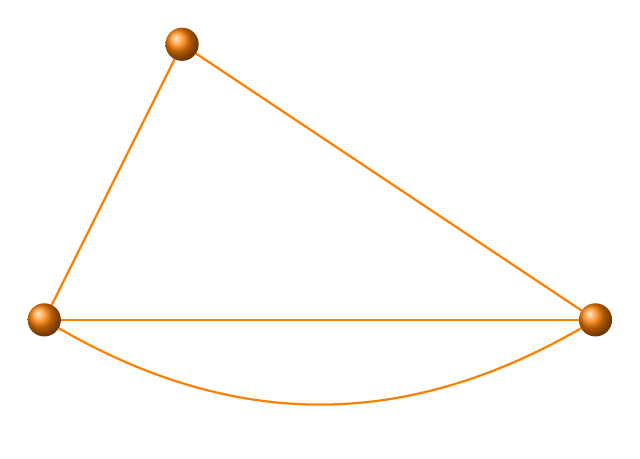
\begin{tikzpicture}[scale=1.75]
  \GraphInit[vstyle=Art]
  \Vertex{A}
  \Vertex[x=4,y=0]{B}
  \Vertex[x=1,y=2]{C}
  \Edge[style={bend left}](B)(A)
  \Edges(A,B,C,A)
\end{tikzpicture}
\end{document}
\end{tkzltxexample}
\end{minipage}
\hfil
\begin{minipage}{.40\textwidth}
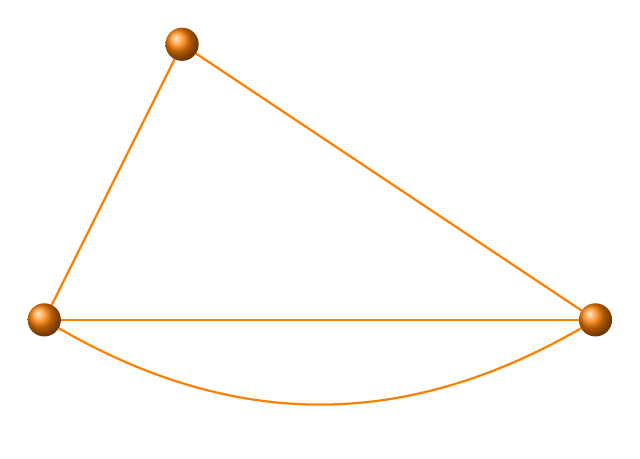
\begin{tikzpicture}[scale=1.75]
  \GraphInit[vstyle=Art]
  \Vertex{A}
  \Vertex[x=4,y=0]{B}
  \Vertex[x=1,y=2]{C}
  \Edge[style={bend left}](B)(A)
  \Edges(A,B,C,A)
\end{tikzpicture}
\end{minipage}

\subsection{A classic example}
The style \tkzname{Normal} is the default one. \tkzcname{Vertices} places a
list of vertices on a circle, \tkzcname{NOEA} places a vertex to the
north-east of another one and \tkzcname{Edges} draws a chain of edges.

\begin{tkzexample}[latex=7cm,small]
\begin{tikzpicture}
  \GraphInit[vstyle=Normal]
  \SetGraphUnit{2}
  \Vertices[rotation=-135]{circle}{A,B,C,E}
  \NOEA[unit=1.414](E){D}
  \Edges(A,B,E,D,C,E,A,C,B)
\end{tikzpicture}
\end{tkzexample}

The same graph with another style:

\begin{tkzexample}[latex=7cm,small]
\begin{tikzpicture}
  \GraphInit[vstyle=Art]
  \SetGraphUnit{2}
  \Vertices[rotation=-135]{circle}{A,B,C,E}
  \NOEA[unit=1.414](E){D}
  \Edges(A,B,E,D,C,E,A,C,B)
\end{tikzpicture}
\end{tkzexample}

\subsection{Loading the package}

\begin{tkzltxexample}[]
\usepackage{tkz-graph}               % or
\usepackage[noshortnames]{tkz-graph}
\end{tkzltxexample}

The package loads \TIKZ\ (with its library \tkzname{arrows}) and
\tkzname{ifthen}. It works with \tkzname{pdflatex}, \tkzname{xelatex} and
\tkzname{lualatex}.

\subsubsection{Short names and prefixed names}
The drawing macros exist under two names:

\medskip
\begin{tabular}{ll}
\toprule
short name & prefixed name \\
\midrule
\tkzcname{Vertex}, \tkzcname{Vertices}  & \tkzcname{tkzVertex}, \tkzcname{tkzVertices} \\
\tkzcname{Edge}, \tkzcname{Edges}, \tkzcname{Loop}
                                        & \tkzcname{tkzEdge}, \tkzcname{tkzEdges}, \tkzcname{tkzLoop} \\
\tkzcname{EA}, \tkzcname{WE}, \tkzcname{NO}, \tkzcname{SO}
                                        & \tkzcname{tkzEA}, \tkzcname{tkzWE}, \tkzcname{tkzNO}, \tkzcname{tkzSO} \\
\tkzcname{NOEA}, \tkzcname{NOWE}, \tkzcname{SOEA}, \tkzcname{SOWE}
                                        & \tkzcname{tkzNOEA}, \tkzcname{tkzNOWE}, \tkzcname{tkzSOEA}, \tkzcname{tkzSOWE} \\
\bottomrule
\end{tabular}

\medskip
Short names like \tkzcname{EA} or \tkzcname{NO} are often used by other
packages or by the user (\tkzcname{EA} is a classic abbreviation of
\tkzcname{expandafter}). For this reason:

\begin{itemize}
\item the prefixed names are always defined;
\item the short names are installed at the beginning of each
      \tkzname{tikzpicture} environment. Outside the pictures, a definition
      of \tkzcname{EA} or \tkzcname{NO} made by the user or by another package
      keeps its meaning;
\item if a short name is already defined when \tkzname{tkz-graph} is loaded,
      a warning gives the prefixed name to use outside the pictures;
\item with the option \tkzname{noshortnames}, the short names are never
      defined.
\end{itemize}

\begin{tkzexample}[latex=7cm,small]
\let\EA\expandafter % user definition
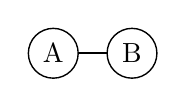
\begin{tikzpicture}
  \Vertex{A} \EA(A){B} % EA of tkz-graph
  \Edge(A)(B)
\end{tikzpicture}

\EA\def\csname test\endcsname{ok}
\test % \EA is \expandafter again
\end{tkzexample}

The macros of settings (\tkzcname{GraphInit}, \tkzcname{tkzSetUpGraph},
\tkzcname{SetUpEdge}\dots) have long names and are always defined.

\subsubsection{Upgrading from version 2.00}
Documents written for the version 2.00 give the same result, with two
exceptions:

\begin{itemize}
\item \tkzname{xkeyval} is no longer loaded: the keys use \tkzname{pgfkeys}.
      A document that uses \tkzname{xkeyval} without loading it must load it.
\item A second \tkzcname{GraphInit}\tkzname{[vstyle=\dots]} in the same group
      was ignored by the version 2.00 (and its value was written in the
      text); it now works.
\end{itemize}

\tkzname{tkz-berge} must be updated at the same time (version 2.2 or later):
the old \tkzname{tkz-berge} needs \tkzname{xkeyval}. The list of all the
changes is in the file \tkzname{CHANGELOG.md}.

\endinput
